Давайте рассмотрим следующую процедуру: для некоторой матрицы $M$ найдём все собственные числа $\lambda_j$, упорядоченные по возрастанию, и определим $r$-параметр \cite{wei_characterization_2020} 
\begin{equation*}
    r \overset{\mathrm{def}}{=}  \left\langle \frac{\min(\delta_j, \delta_j+1)}{\max(\delta_j, \delta_{j+1})} \right\rangle_j,
    \hspace{10 mm} 
    \delta_j = \lambda_{j+1}-\lambda_j.
\end{equation*}
Сразу можем отметить несколько таких свойств, что он не чувствителен к преобразованиям вида $M \to \alpha_1 M + \alpha_2 \1$, более того как позже заметим он много к чему не чувствителен. 


\begin{figure}[tb]
    \centering
    \addletter{107}{a}
    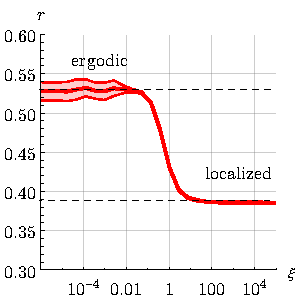
\includegraphics[width=0.225\textwidth]{imgs/erg_reg_add1.pdf}
    \hspace{10 mm} 
    \addletter{107}{b}
    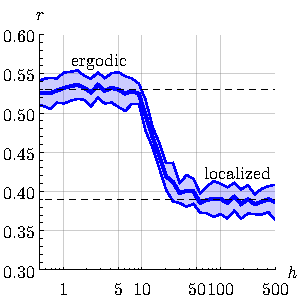
\includegraphics[width=0.225\textwidth]{imgs/erg_reg_add2.pdf}
    \caption{a) Phase transition EP-LP with random matrix. b)  Phase transition EP-LP with 1D hard-bosons \eqref{9:model}, $h \equiv \Delta$}
    \label{fig:rxi}
\end{figure}


Теперь посмотрим подробнее на систему \eqref{9:model} и фазовый переход, который случается при повышении $\Delta$. В координатном представлении шумы являются просто случайной диагональной добавкой к гамильтониану\footnote{
    Тут нужно быть аккуратным, потому что как мы увидим позднее, небольшим изменения диагонали через $V \neq 0$ приводят к принципиально другому поведению системы \cite{bardarson_unbounded_2012}. 
}. Таким образом при $\Delta \gg J$ (по крайней мере в одночастичном случае) гамильтониан практически диагонализуется (fig. \ref{fig:loc1}). С другой стороны есть недиагональная часть, за которую отвечает $J$. В статье \cite{wei_characterization_2020} предлагается моделировать этот фазовый переход с помощью двух случайных матриц: случайной эрмитововой $M_1$ (GOE) и случайной диагональной $M_2$, таким образом $M = (1-k) M_1 + k M_2$. The limiting values $k=0$ and $k=1$ characterize chaotic and nonchaotic regimes (термализующийся и локализующийся). Чтобы переход не зависел от параметров $M_{1,2}$ можем scale $k$ as
\begin{equation*}
    \xi = \frac{1}{D} \frac{k \sigma_2}{(1-k)\sigma_1},
\end{equation*}
where $\sigma_{1,2}$ are the standard deviation of elements in $M_{1,2}$ respectively and $D$ is the size of the matrix. 

Найдём, как зависит $r(\xi)$ для матриц при $D=200$, $\sigma_1=\sigma_2=1$ (для других значений зависимость такая же), усредняя результат по 100 реализациям (fig. \ref{fig:rxi}a). Для сравнения приведена зависимость $r(\xi)$ для 1D системы \eqref{9:model} hard-bosons по уровню шума $h$ (то же самое, что и $\Delta$) на решётке в $L=14$ узлов с половинным заполнением\footnote{
    Если бы мы говорили про Heisenberg model, то это соотвествовало полному спину равному нулю. 
} (7 частицами).  В соответсвии с \cite{wei_characterization_2020, pal_many-body_2010} значение $r \approx 0.53$ является маркером эргодической фазы (характерное значение для GOE), а $r \approx 0.39$ является маркером локализованной фазы (так называемая Poisson statistics):
\begin{equation*}
\boxed{
    r \approx 0.53 \text{ -- ergodic}
}
\hspace{10 mm} 
\boxed{
    r \approx 0.39 \text{ -- localized}
}
\end{equation*}
Замечу, что используется именно слово маркер, так как эти условия не являются необходимыми и не являются достаточными. 

\begin{figure}
    \centering
    \addletter{50}{a}
    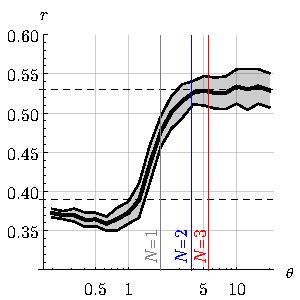
\includegraphics[align=c, width=0.225\textwidth]{imgs/ergodic_reg.pdf}
    \hspace{10 mm} 
    \addletter{50}{b}
    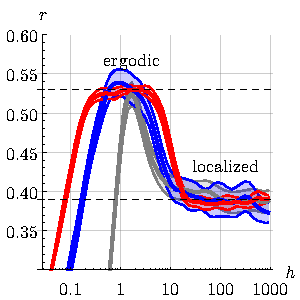
\includegraphics[align=c, width=0.225\textwidth]{imgs/transition.pdf}
    \hspace{5 mm} 
    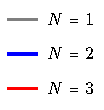
\includegraphics[align=c, width=0.075\textwidth]{imgs/transition_leg.pdf}
    \caption{
        a) The influence of matrix rarefaction $\theta$ on phase formation. 
        b) Phase transition with 1D hard-bosons 
    % N=200
    % $\xi=0.01$, $L=20$
    }
    \label{fig:rtheta}
\end{figure}

 

% \cite{pal_many-body_2010} -- The many-body localization phase transition


Аналогичная зависимость получится, если в качестве $M_1$ будем рассматривать матрицу связности случайного графа (эрмитова матрица со случайными элементами $0,1$). 
Считая, что в среднем на строчку приходится $\theta$ ненулевых элементов, можем задаться вопросом о влиянии $\theta$ на формировании эргодической фазы (fig. \ref{fig:rtheta}a). При слишком маленьких $\theta$ высока вероятность Hilbert Space Fragmentation \cite{Moudgalya_2022}, что очевидно не может давать термализацию системы. Тем более система не термализуется, когда является интегрируемой \cite{rigol_thermalization_2008}.

Такое внимание к $\theta$ и фрагментации уделил, так как это в каком-то смысле помогает понять, почему для небольшого числа частиц в системе эргодическая фаза (судя по $r$) практически не наступает (fig. \ref{fig:rtheta}). Действительно, при меньшем числе частиц ($N=1,2,3$) и том же размере решётки $L=14$ гамильтониан более разряженный (fig. \ref{fig:rtheta}a), происходит Hilbert Space Fragmentation (то есть гамильтониан можно представить в блочно диагональном виде) и, соответсвенно, не происходит термализации. 


Основной вывод этого раздела: $r$-параметр носит достаточно универсальный характер, может использоваться как маркер эргодичной фазы и локализованной фазы. Фазовый переход EP-LP может моделироваться случайными матрицами (GOE, random diagonal, random graph adjacency matrix).